\documentclass[12pt]{standalone}
\usepackage{tikz}
\usetikzlibrary{positioning}
\begin{document}
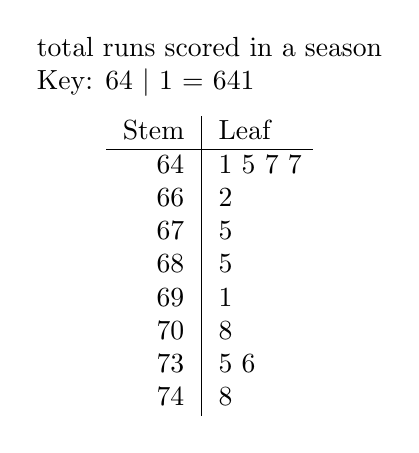
\begin{tikzpicture}
\node[align=left] (top_node) at (0,0){total runs scored in a season \\ Key: 64 $\vert$ 1 = 641};
\node[below=of top_node,yshift=10mm] {
\begin{tabular}{r|l@{\hspace{4 pt}}}
Stem & Leaf\\
\hline
64 & 1 5 7 7 \\66 & 2 \\67 & 5 \\68 & 5 \\69 & 1 \\70 & 8 \\73 & 5 6 \\74 & 8 \\
\end{tabular}};
\end{tikzpicture}
\end{document}